\section{Opis}
\subsection{Perspektiva proizvoda}
Bulletinboard je samostalna web aplikacija koja sadrži svoju bazu smještenu na odvojenom računaru (serveru) i za pristup aplikaciji je neophodna Internet konekcija.
\subsection{Funkcionalnosti proizvoda}
\subsubsection{Bulletinboard profil}
Bulletinboard profil omogučava sljedeče pogodnosti:
\begin{itemize}
    \item Odličan način praćenja personalnog progresa
    \item Efektivno organizovanje vremena i taskova
    \item Mjesto za pregled odabranih sadržaja
    \item Mjesto za efektivno informisanje
    \item Brzo dijeljenje potrebnog sadržaja sa društvenih mreža
    \item Poticanje inspiracije, efikasnosti i kreativnosti
    \item Povećava interesovanje i motivaciju
    \item Kalendarsku organizaciju vremena
\end{itemize}

\subsubsection{Administracija korisnika}
Upravljanje klijentima zahtijeva privilegovani pristup administratora, a uključuje:
\begin{itemize}
    \item Kreiranje novog korisnika
    \item Modifikacija postojećeg korisnika
    \item Brisanje postojećeg korisnika
    \item Opcija ban-ovanja (zabrana pristupa korisniku)
    \item Pretraga i pregled korisnika
\end{itemize}

\subsection{Karakteristike korisnika}
Svi korisnici imaju iste mogućnosti upotrebe aplikacije. Izdvajaju se administratori sistema koji su zaduženi za održavanje korisničkih računa.
\subsubsection{Mogućnosti korisnika}
Korisnik sistema ima sljedeće mogućnosti:
\begin{itemize}
    \item Prijava na sistem
    \item Odjava sa sistema
    \item Kreiranje neovog korisničkog računa
    \item Dodavanje slike
    \item Brisanje slike
    \item Dijeljenje sadržaja sa društvenih mreža
    \item Dodavanje posta
    \item Brisanje posta
    \item Dodavanje posta sa datumom(kalendar)
\end{itemize}
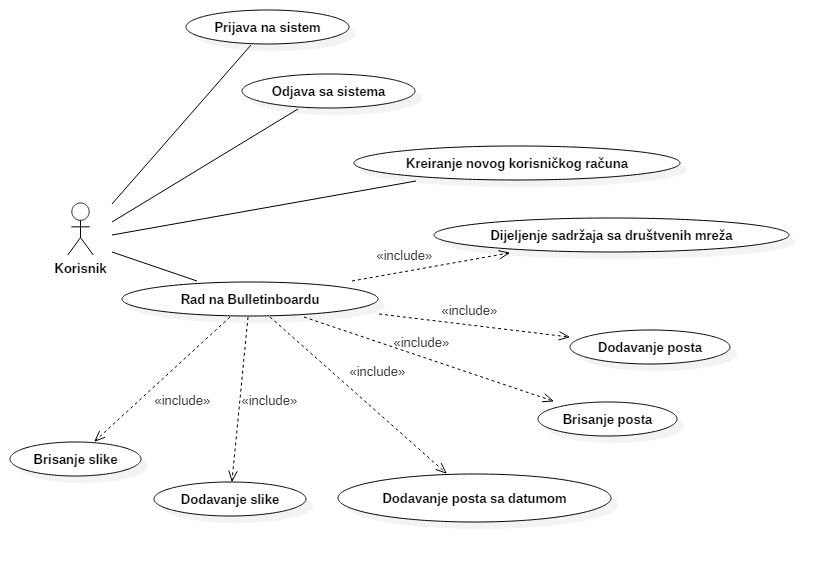
\includegraphics[scale=0.5]{SRS/use_cases/korisnik_use_case.png}

\subsubsection{Mogućnosti administratora}
Administrator sistema ima sljedeće mogućnosti:
\begin{itemize}
    \item Brisanje korisnika
    \item Pretraga i pregled korisnika
    \item Modifikacija korisnikovog profila
    \item Zabrana pristupa korisniku (ban)
    \item Održavanje sistema i korekcija grešaka
    \item Kreiranje izvještaja
    \item Pregled pinova koji imaju najveci broj djeljenja na mrežama
\end{itemize}
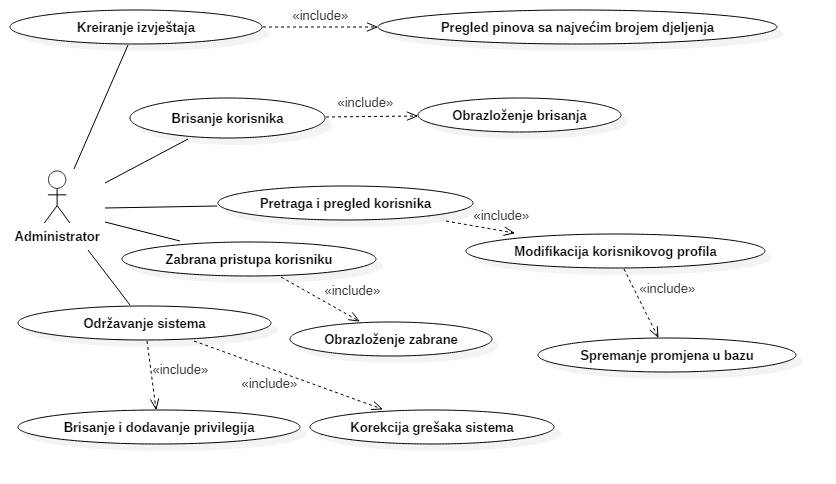
\includegraphics[scale=0.5]{SRS/use_cases/admin.png}
\subsection{Ograničenja}
\subsubsection{Zakonska ograničenja}
Zakonska ograničenja za ovaj sistem ne postoje. Postovi ne dozvoljavaju dijeljenje datoteka ili medijskog sadržaja, tako da sistem ne podliježe pravilnicima o zaštiti autorskih prava. Društvene mreže sa kojih je moguće dijeliti sadržaj u svojim pravima korištenja dozvoljavaju dijeljenje sadržaja, tako da tu ne postoje zabrane na koje je potrebno obratiti pažnju. U skladu sa navedenim, zaključuje se kako lokacija aplikacije nije ograničena lokalnim zakonima.
\subsubsection{Hardverska ograničenja}
Korisnički računari nemaju hardverska ograničenja. Potrebno je posjedovanje dovoljne konfiguracije za pokretanje web preglednika koji podržava novije internet protokole.

Za instalaciju servera i baze podataka koristit će se centralni računar sa minimalnom konfiguracijom:

\begin{itemize}
    \item Radna frekvencija procesora (CPU): 2.40GHz
    \item Količina RAM memorije: 4GB
    \item Količina memorije za trajno skladištenje (HDD): 500 GB
\end{itemize}

Po dogovoru sa klijentom, usluga se iznajmljuje od Cloud Operatera. Prilikom sklapanja ugovora sa pružaocem usluge Cloud Hostinga, preporučuje se konfiguracija virtualne mašine kakva je predviđena iznad ili bolja.

Za uspostavljanje izlaza na internet koristi će se mrežni kablovi, te sljedeći mrežni uređaji:
\begin{itemize}
  \item Switch: 10/100/1000 Mbps
  \item Ruter: 10/100 Mbps
\end{itemize}

Bitno je napomenuti kako konekciju na internet održava ISP i potrebna je stalna internet konekcija za pristup aplikaciji.
\subsubsection{Softverska ograničenja}
Korisnici aplikaciji mogu pristupiti putem jednog od sljedećih internet pretraživača: Firefox 52+, Chrome, Microsoft Edge.

Na serverskoj strani je potrebno obezbijediti MongoDB bazu podataka te operativni sistem sa instaliranim JRE (Java SE Runtime Environment) 8, ili novijim.

\subsection{Pretpostavke i zavisnosti}
\begin{itemize}
    \item \textbf{Pretpostavka 1.} Pretpostavlja se da se radi na novom informacionom sistemu, a ne na nadogradnji postojećeg. Nije potrebno raditi integraciju sa postojećim komponentama i prilagođavati se postojećem sistemu.
    \item \textbf{Pretpostavka 2.} Pretpostavlja se da je moguće nabaviti hardverske resurse potrebne za održavanje stranice aktivnom. Preporučeno je da se te usluge iznamljuju od cloud providera putem virtuelnih mašina.
    \item \textbf{Pretpostavka 3.} Pretpostavlja se da hardver ima instaliran potreban softver naveden u poglavlju "Softverski zahtjevi". Neki dijelovi softvera imaju licence za slobodno korištenje, dok je za druge potrebno platiti korištenje.
    \item \textbf{Pretpostavka 4.} Pretpostavlja se da serverski računari imaju svu potrebnu fizičku zaštitu. Ukoliko se koristi hardver cloud providera takvi uslovi se podrazumijevaju sklapanjem ugovora sa pružaocem usluge. Ukoliko se koristi vlastiti hardver, potrebno je osigurati dovoljan nivo zaštite da se server i rad sistema ne dovede u opasnost.
    \item \textbf{Pretpostavka 5.} Pretpostavlja se da serverski računar ima obezbijeđeno stabilno napajanje u svakom trenutku (24h dnevno). Prilikom sklapanja ugovora sa pružaocem cloud hosting usluge, dogovara se procenat vremena u kojem je usluga dostupna. Ukoliko se koristi vlastiti hardver, potrebno je osigurati UPS uređaje koji pružaju mogućnost napajanja u kriznim situacijama, kako bi sistem mogao nesmetano raditi.
    \item \textbf{Pretpostavka 6.} Preetpostavlja se da korisnici sistema imaju dovoljne hardverske konfiguracije za pristupanje web aplikaciji.
    \item \textbf{Pretpostavka 7.} Pretpostavlja se da korisnici sistema posjeduju osnovno poznavanje rada na računaru, pristupa i korištenja interneta.
    \item \textbf{Pretpostavka 8.} Pretpostavlja se da pristup serverskom računaru sa centralnom bazom podataka nema niko osim ovlaštene osobe, te da ovlaštena osoba neće zloupotrijebiti svoj položaj i vršiti manipulacije nad zapisima u bazi podataka. Ukoliko je sklopljen ugovor sa pružaocem cloud usluge, pretpostavlja se da će pružaoc poštovati stavke ugovora o čuvanju privatnosti i ograničenju neovlaštenog pristupa.
    \item \textbf{Pretpostavka 9.} Pretpostavlja se da ukoliko u toku ili nakon izrade sistema dođe do promjene zahtjeva ili dodatnih zahtjeva za funkcionalnostima, potrebno je pratiti korake koji su navedeni u poglavlju 2.6. Planiranje zahtjeva ovog dokumenta.
\end{itemize}
\subsection{Planiranje zahtjeva}
Kao početni dio razvoja softvera i cjelokupnog informacionog sistema, rade se faze analize zahtjeva i dizajna. Prvenstveno se radi analiza funkcionalnih i nefunkcionalnih zahtjeva, kao i navedenih ograničenja (zakonskih, hardverskih, softverskih). U slučaju eventualnih promjena zahtjeva potrebno je pratiti ustaljenu proceduru opisanu sljedećim koracima:
\begin{itemize}
    \item Od naručioca sistema se zahtjeva da dostavi zvanični zahtjev za promjenu funkcionalnosti sa detaljno opisanim traženim funkcionalnostima i promjenama nad sistemom.
    \item SI Pinboard Team se obavezuje da će u najkraćem roku od prijema zahtjeva uraditi analizu traženih promjena i dostaviti odgovor u vidu ponude koja opisuje mogućnost izvedbe traženih funkcionalnosti.
    \item Ukoliko je ponuda prihvatljiva, SRS se revidira i postaje nova, važeća, verzija dokumenta.
\end{itemize}

U slučaju da dođe do promjene zahtjeva nakon zaključivanja specifikacije, razvojni tim zadržava pravo na ne izvršavanje traženih promjena.

U slučaju da razvojni tim ima prijedlog na postojeće funkcionalnosti sistema nakon zaključivanja specifikacije, potrebno je pratiti ustaljenu proceduru opisanu sljedećim koracima:
\begin{itemize}
    \item Od razvojnog tima se zahtjeva da dostavi zvaničnu promjenu funkcionalnosti sa detaljno opisanim traženim funckcionalnostima i promjenama nad sistemom uključujući i utjecaj koji promjene imaju na vrijeme i cijenu razvoja.
    \item Naručilac sistema je dužan u roku 15 dana donijeti zaključak o predloženim izmjenama.
    \item Ukoliko je ponuda prihvatljiva, SRS se revidira i postaje nova, važeća, verzija dokumenta.
\end{itemize}
